\section{Methodology and Test Framework}
\label{sec:methodology}

A dual-rate framework separates continuous-time physics
($f_{\mathrm{s,phys}}=1$\,MHz) from DSP estimation ($f_{\mathrm{s,DSP}}=10$\,kHz,
ratio $100{:}1$), reproducing relay-class sampling constraints with
negligible numerical error. Throughout, $\omega$ denotes angular frequency
(rad/s); $f = \omega/2\pi$ in Hz or mHz.
% ---------------------------------------------------------
\subsection{Evaluated Estimators}
% ---------------------------------------------------------

Twelve estimators from five algorithmic families are evaluated
(Table~\ref{tab:unified_2024_big}).
\textbf{Loop-based:} SRF-PLL and a bandpass-pre-filtered SOGI-FLL.
The SOGI-FLL departs from the textbook formulation~\cite{Golestan2015}
through two additions: an IIR bandpass pre-filter at 50\,Hz that suppresses
harmonic contamination before the SOGI core, and a FastRMS adaptive normalizer
that compensates amplitude variations. A $2\pi$-scaling error in the standard
adaptation law (gain mis-scaled by ${\approx}377\times$) was corrected before
evaluation; results are therefore not directly comparable to published SOGI-FLL
figures. The resulting narrow passband suppresses apparent frequency deviation
under phase jumps but cannot track sustained RoCoF, explaining the divergent
ranking across Scenarios~B and~D.
\textbf{Window-based:} IpDFT with a Hann window and three-point
magnitude-parabolic interpolation~\cite{Quinn1994}; TFT with a 2nd-order
Taylor-Fourier model, Hann-weighted, providing improved RoCoF tracking at
the cost of higher noise sensitivity~\cite{PlatasGarza2011}.
\textbf{Adaptive recursive:} RLS and VFF-RLS with AR(2) bandpass pre-whitening.
\textbf{Data-driven:} Koopman (RK-DPMU) and PI-GRU.
\textbf{Model-based:} EKF, UKF, and RA-EKF (``RoCoF Out.'': S\,=\,explicit
state, D\,=\,finite-difference). The UKF applies a 10-sample output moving
average ($+0.5$\,ms group delay), which marginally improves steady-state
RMSE at the cost of transient settling time.

The RA-EKF extends the 3-state EKF with an explicit RoCoF state,
$\mathbf{x}_k = [\theta_k,\omega_k,A_k,\dot{\omega}_k]^\top$, and two
IBR-specific mechanisms~\cite{Ferrero2020EKF,Chamorro2021}.
\emph{Innovation-Driven Covariance Scaling} scales the process noise matrix
by the normalised innovation magnitude, inflating $\mathbf{Q}_k$ during
transients and shrinking it at steady state.
\emph{Event Gating} soft-resets only $\theta_k$ when the innovation exceeds
$\gamma\hat{\sigma}_\nu$ ($\gamma\!=\!2.0$), preserving $\omega_k$ and
$\dot{\omega}_k$ to bound cycle-slip at phase discontinuities.

% ---------------------------------------------------------
\subsection{Test Scenarios and Noise Model}
\label{sec:scenarios}
% ---------------------------------------------------------

Five scenarios stress the estimators under IBR-grid conditions
(Fig.~\ref{fig:scenarios}). Ground-truth frequency is the analytical
time derivative of the phase signal; this produces a non-flat trajectory
after phase jumps. Noise levels: AWGN $\sigma=0.001$\,pu for (A)--(C),
$0.005$\,pu for (D), and $0.003$\,pu with sparse impulsive samples
($\leq\!0.05$\,pu, $<\!1\%$ rate) for (E).
%
\begin{itemize}[leftmargin=*, nosep, topsep=1pt, itemsep=1pt]
  \item[\textbf{(A)}] \textbf{Magnitude Step:} $+10\%$ voltage step with
    zero phase angle at the disturbance onset.
  \item[\textbf{(B)}] \textbf{Frequency Ramp:} $+3.0$\,Hz/s RoCoF (IEEE 1547-2018 Category III compliant).
  \item[\textbf{(C)}] \textbf{AM Modulation:} 10\% depth at 2\,Hz.
  \item[\textbf{(D)}] \textbf{Composite Islanding:} instantaneous
    $+60^\circ$ phase jump~\cite{Roscoe2019}, 5th/7th harmonics (4\%/2\%),
    0.5\% 32.5\,Hz interharmonic~\cite{Bernal2024,Zoghby2024}
    (THD\,$\approx$\,4.5\%, IEEE~519 compliant), $\sigma=0.005$\,pu noise.
  \item[\textbf{(E)}] \textbf{IBR Multi-Event:} 5\,s sequence with
    harmonic-rich steady state (5th: 4\%, 7th: 2\%;
    THD\,$\approx$\,4.5\%, IEEE~519 compliant), a $+40^\circ$
    phase jump, a $-3.0$\,Hz/s RoCoF segment reaching a nadir of
    $57.5$\,Hz (IEEE~1547-2018 UFLS limit), a $+80^\circ$ jump with
    second-order ring-down recovery, and impulsive noise~\cite{Chamorro2021}.
  \item[\textbf{(F)}] \textbf{Primary Frequency Response} (\emph{planned extension}):
    a second-order electromechanical recovery following a generation loss
    event, modelling governor--turbine dynamics with damping. Monte Carlo
    evaluation under this scenario is reserved for future work.
\end{itemize}
%
Scenarios~(A)--(C) follow the IEC/IEEE~60255-118-1 test philosophy,
whereas Scenarios~(D)--(E) introduce IBR-specific disturbances beyond
the standard scope.

% ---------------------------------------------------------
\subsection{Performance Metrics and Optimization Protocol}
\label{sec:metrics}
% ---------------------------------------------------------

Scenario-wise grid search (Table~\ref{tab:hyperparams}) minimizes RMSE
per estimator--scenario pair, establishing the \emph{performance ceiling}
of each family independently. PI-GRU is a fixed pre-trained baseline;
all classical methods are scenario-optimized. Monte Carlo robustness uses
$N\!=\!30$ runs per pair (seeds 2000--2029; tuning seed: 42).
Let $e(t)=\hat{f}(t)-f_{\mathrm{true}}(t)$.
Four metrics quantify performance: \textbf{RMSE},
\textbf{Peak Error} ($|e|_{\max}$),
\textbf{Settling Time} (first time $|e|\leq\!200$\,mHz sustained for
$\geq\!20$\,ms), and \textbf{Trip-Risk Duration} ($T_{\mathrm{trip}}$:
cumulative time with $|e|>0.5$\,Hz).
Computational cost is mean time per sample over 20 timed repetitions
(Python~3.13, Intel Core Ultra 5 125H, single-threaded); reported values
are Python baselines for relative comparison only---C/FPGA implementations
yield 10--100$\times$ lower latencies. IpDFT structural latency equals
$N_c/f_0 = 33$--$167$\,ms (observation delay, not stochastic lag).

The compliance heatmap (Fig.~\ref{fig:dashboard_mega}g) applies
IEC/IEEE~60255-118-1-derived thresholds: RMSE\,$<$\,50\,mHz,
peak\,$<$\,500\,mHz, $T_{\mathrm{trip}}<0.1$\,s (visualization only;
no certification implied). \textbf{F*} marks marginal failure: RMSE
overshoot $<\!1.5\%$ above threshold or a sub-cycle peak exceedance only.

\begin{table}[b!]
  \centering
  \scriptsize
  \setlength{\tabcolsep}{3pt}
  \caption{Tuning Parameter Search Space (${\approx}5{,}000$ total runs).
    \emph{log}: 12 log-spaced pts/decade; \emph{linear}: 10 pts;
    $\{\cdot\}$: discrete set.
    Units: $K_p$~[pu/rad], $K_i$~[pu/(rad$\cdot$s)], $R$~[pu$^2$],
    $N_c$~[cycles], $N_{\mathrm{smooth}}$~[samples].}
  \label{tab:hyperparams}
  \begin{tabular}{l l p{4.5cm}}
    \toprule
    \textbf{Method} & \textbf{Param.} & \textbf{Search Range (spacing; \# pts)} \\
    \midrule
    SRF-PLL      & $K_p$, $K_i$
                 & $[1,60]$, $[1,200]$ (linear, 10 pts each) \\
    EKF / RA-EKF & $Q$
                 & $10^{-4}$--$10^{4}$ (log, 12 pts) \\
                 & $R$
                 & $10^{-5}$--$10^{0}$ (log, 12 pts; $R_{\max}=1.0$) \\
    RA-EKF only  & $\hat{\sigma}_\nu$, $\gamma$
                 & $\{0.1,0.3\}$, $2.0$ (fixed; 2 pts / 1 pt) \\
    SOGI-FLL     & $k$, $g_{\rm FLL}$
                 & $\{0.5,1.0,1.5,2.0\}$, $\{5,10,\ldots,150\}$ \\
    IpDFT        & $N_c$
                 & $\{2,3,4,6,8,10\}$ cycles (6 pts) \\
    RLS / VFF    & $\lambda$, $N_{\mathrm{smooth}}$
                 & $0.9$--$0.99999$ (log, 12 pts), $2$--$2000$\,samp. (log, 10 pts) \\
    TFT          & $N_c$
                 & $\{2,3,4,6\}$ cycles (4 pts) \\
    TKEO         & Smooth window
                 & $10$--$50$\,samples (linear, 9 pts) \\
    \bottomrule
  \end{tabular}
\end{table}


\begin{figure*}[t!]
    \centering
    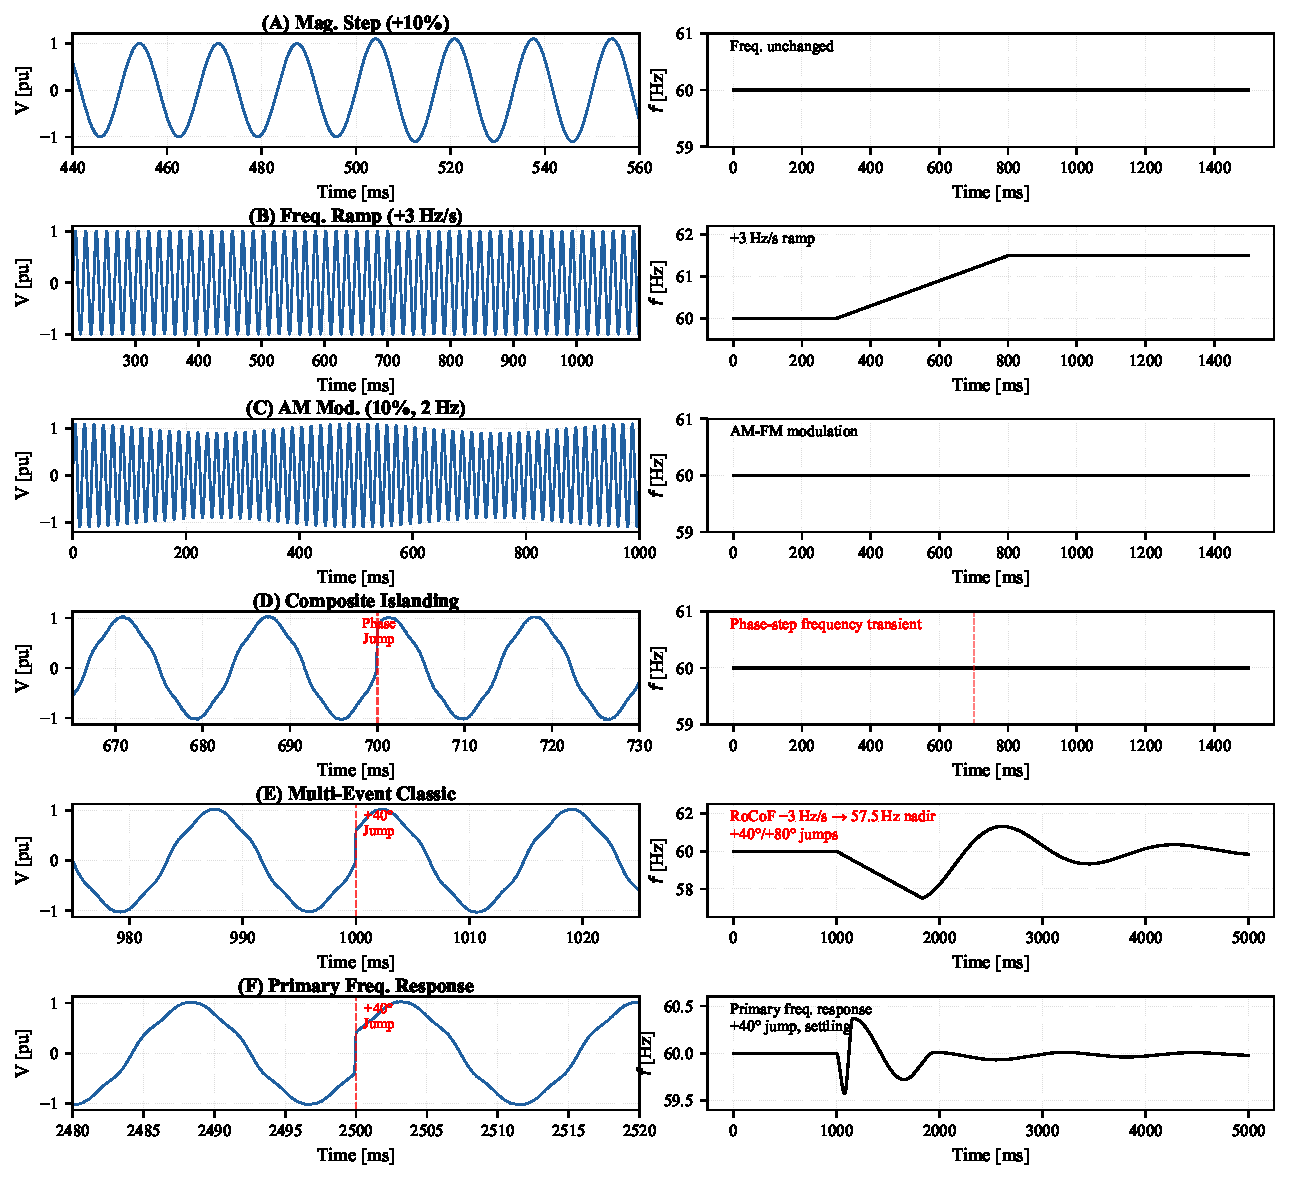
\includegraphics[width=0.99\textwidth]{Figures/Plots_And_Graphs/Fig1_Scenarios_Final.pdf}
    \caption{Complete Stress-Test Scenario Suite. (A–C) Dynamic performance
        profiles following the test philosophy of IEC/IEEE~60255-118-1
        (step, ramp, modulation). (D) Composite Islanding featuring an
        instantaneous $+60^\circ$ phase jump with harmonics and elevated noise
        ($\sigma = 0.005$\,pu; Section~\ref{sec:scenarios}).
        (E) IBR Multi-Event: scenario-dependent noise ($\sigma_\text{base}=0.003$\,pu
        plus sparse impulsive spikes $\leq 0.05$\,pu); frequency profile shows
        the full 5\,s composite sequence.}
    \label{fig:scenarios}
\end{figure*}